\section*{Goldsponsor und Aussteller}
%\begin{center}
  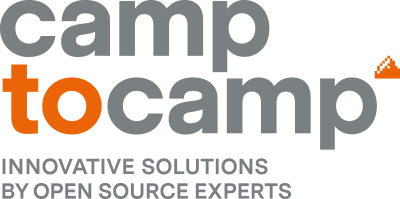
\includegraphics[width=0.8\textwidth]{101_camptocamp.png}
  %\end{center}
  \vspace{1.0\baselineskip}
  
\noindent
    {\bfseries CamptoCamp}\\
    Camptocamp gehört zu den führenden Dienstleistern im Bereich Open Source GIS mit starkem Engagement in den unterschiedlichen Communities.

 \noindent   
Unsere Dienstleistungen stützen sich auf über 20 Jahre Erfahrung in der Umsetzung von innovativen GIS-Lösungen für Behörden und Unternehmen. Unser Leitmotiv ist ein hochwertiger, auf die Anforderungen des Kunden zugeschnittener Service. Das Besondere an Camptocamp sind die hochqualifizierten Mitarbeitenden und ihr grosses Engagement im Ökosystem Open Source GIS. Camptocamp ist Initiator und Hauptbeitragender der Open Source Projekte GeoServer-Cloud, GeoNetwork-UI und MapFish-Print. Für die oft anspruchsvollen Projekte unserer Kunden entwickeln wir massgeschneiderte Lösungen auf Basis modernster Open-Source-Technologien.

 \noindent   
Camptocamp ist in München, Bussigny, Olten, Chambéry und Paris vertreten. Neben Lösungen im GIS-Bereich bieten wir auch eine grosse Expertise in den Bereichen ERP Enterprise-Resource-Planning und IT-Infrastruktur.
